See Tables \ref{eq:solutions/3/7/7/table:1} and \ref{eq:solutions/3/7/7/table:1}


\begin{table}[!ht]
	\begin{center}
		\begin{tabular}{|c|c|}
			\hline
			& \\
			& \\
			\textit{iso-} & A linear transformation $T : V\rightarrow W$\\
			\textit{morphism} & is $\textit{isormorphism of}$ $V$ $\textit{onto}$ $W$\\
			& if $T$ is $one-one$\\
			& \\
			\hline	
			& \\		
			\textit{one-one} & A linear transfrmation $T : \mathbb{R}^{n} \rightarrow \mathbb{R}^{m}$\\
			& is $\textit{one-one}$\\
			& if $\forall \vec{b} \in \mathbb{R}^{m}$,  $\vec{A}\vec{X} =\vec{b}$\\
			& has at most one solution in $\mathbb{R}^{n}$\\
			& \\
			& By definition, all $invertible$\\
			& linear transformations are $\textit{one-one}$\\
			& \\
			\hline
			& \\
			\textit{invertible} & A linear transformation $T : V \rightarrow W$\\
			& is $\textit{invertible}$ if there exists another\\
			& linear transformation $U: W \rightarrow V$\\
			& such that\\
			& $UT$ is identity transformation on $V$\\
			& and \\
			& $TU$ is identity transformation on $W$\\
			& \\
			\hline
		\end{tabular}
	\end{center}
\caption{Definitions}
\label{eq:solutions/3/7/7/table:1}
\end{table}
\begin{figure}[!ht]
\centering
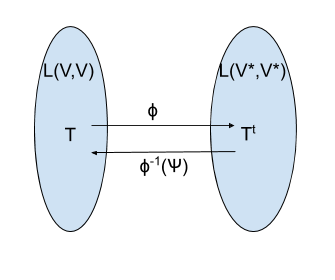
\includegraphics[width=\columnwidth]{solutions/3/7/7/fig/transpose.png}
\caption{$\enspace \phi : L(V,V) \rightarrow L(V^*,V^*)$}
\end{figure}
\begin{table}[!ht]
\begin{center}
\begin{tabular}{|c|c|}
\hline
& \\
Given & $\phi(T) = T'$ where\\
& $\phi : L(V,V) \rightarrow L(V^*,V^*)$\\
& $T \in L(V,V)$ and $T' \in L(V^*,V^*)$\\
& \\
\hline
& \\
To prove & $\phi$ is an $isomorphism$ of\\
& $L(V,V) \enspace onto \enspace L(V^*,V^*)$\\
& $i.e \enspace \phi \text{ is } one-one \implies \phi$ is \textit{invertible}\\
& \\ 
\hline
& \\
Proof & Consider a linear transformation\\
& $\psi : L(V^*,V^*) \rightarrow L((V^*)^*,(V^*)^*)$\\
& \\
& We know, $L((V^*)^*,(V^*)^*) = L(V,V)$\\
& \\
& Hence $\psi : L(V^*,V^*) \rightarrow L(V,V)$\\
& \\
& We have $\phi \circ \psi = I$ and $\psi \circ \phi = I$\\
& \\
& $\therefore$ $\phi$ is invertible with $\psi$ its inverse.\\
& \\
& Hence $\phi$ is $\textit{isomorphic}$.\\
& \\
\hline
\end{tabular}
\end{center}
\caption{Solution}
\label{eq:solutions/3/7/7/table:2}\end{table}

{\em Example}
Consider, $T \in L(\mathbb{R}^3,\mathbb{R}^3)$
\begin{align}
	T &= \myvec{2 & 1 & 1\\ 1 & 1 & 0\\ 0 & 0 & 1} \text{ and }\\
	T' &= \myvec{2 & 1 & 0\\1 & 1 & 0\\1 & 0 & 1}
\end{align}
If $T \in L(\mathbb{R}^3,\mathbb{R}^3)$ we can show that $T' \in L({\mathbb{R}^3}^*,{\mathbb{R}^3}^*)$ as follows.\\ 
\\Consider linear functional $f : {\mathbb{R}^3}^* \rightarrow F$ 
\begin{align}
	f(x,y,z) = 2x + 3y + 4z
\end{align}
Let $g : \mathbb{R}^3 \rightarrow F$. By definition of transpose,
\begin{align}
	g &= T'f\\
	&= \myvec{2 & 1 & 0\\1 & 1 & 0\\1 & 0 & 1}\myvec{2\\3\\4} = \myvec{7\\5\\6}\\
	g(x,y,z) &= 7x + 5y + 6z
\end{align}
\begin{figure}[!ht]
\centering
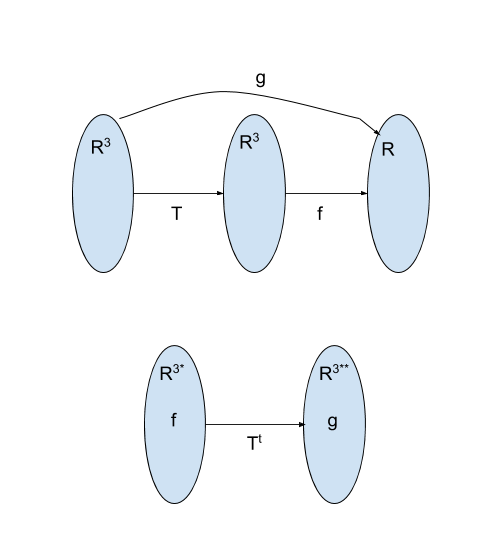
\includegraphics[width=\columnwidth]{solutions/3/7/7/fig/transpose_example.png}
\caption{$T: \mathbb{R}^3 \rightarrow \mathbb{R}^3$ and $T': {\mathbb{R}^3}^* \rightarrow {\mathbb{R}^3}^{**}$}
\end{figure}
Consider vector in $v = \myvec{1\\2\\3} \in \mathbb{R}^3$,
\begin{align}
	Tv &= \myvec{2 & 1 & 1\\ 1 & 1 & 0\\ 0 & 0 & 1}\myvec{1\\2\\3} = \myvec{7\\3\\3}\\
	f(Tv) &= f(7,3,3)\\
	 &= 2*7 + 3*3 + 4*3 = 35\\
	 g(1,2,3) &= 7*1 + 5*2 + 6*3 = 35 
\end{align}
Hence verified $g = T'f$, and $T'$ is transpose of $T$. \\
\\
Now we will show that $\phi$ is invertible. 
Given,
\begin{align}
	\phi T &= T'\\
	\phi &= T'T^{-1}\\
	&= \myvec{2 & 1 & 0\\1 & 1 & 0\\1 & 0 & 1}\myvec{2 & 1 & 1\\ 1 & 1 & 0\\ 0 & 0 & 1}^{-1}\\
	&= \myvec{2 & 1 & 0\\1 & 1 & 0\\1 & 0 & 1}\myvec{1 & -1 & -1\\-1 & 2 & 1\\0 & 0 & 1}\\
	\phi &= \myvec{1 & 0 & -1\\0 & 1 & 0\\0 & 0 & 1}\\
	\phi^{-1} &= \myvec{1 & 0 & -1\\0 & 1 & 0\\0 & 0 & 1}^{-1} = \myvec{1 & 0 & 1\\0 & 1 & 0\\0 & 0 & 1}
\end{align}
Since $\phi^{-1}$ exists, $\phi$ is isomorphism of $L(V,V)$ onto $L(V^*,V^*)$
